\section{\textbf{EnDASH System}}\label{sec:chap04:sys_overview}
The proposed EnDASH system is an energy efficient client video player, working as a wrapper over \ac{DASH}. It predicts the cellular network throughput over a finite future time window to take decisions on the opportune fetching of  video chunks.  EnDASH operates in a time-slotted fashion. So, the entire timeline is divided into discrete time-slots of length \mq{T}.
EnDASH executes the following functions to achieve energy efficient video download: (i) At the beginning of each time slot it uses historical data on radio parameters to predict the cellular network link throughput of the current time slot using a Random Forest Learning (RFL) engine. (ii) It then uses the predicted throughput to predict the optimal playback-buffer length for the current slot that minimizes energy consumption. For this, EnDASH employs the state-of-the-art \ac{A3C} deep \ac{RL} algorithm.  (iii) Before downloading each video chunk within a time slot, EnDASH runs another A3C based deep \ac{RL} engine to predict the optimal download chunk  bitrate. 
EnDASH is, thus, a cascaded system of three engines: (i) throughput prediction, (ii) buffer length decision,  and (iii) bitrate selection as shown in \fig\ref{fig:chap04:EnDASH system}. We next describe these modules.
 \begin{figure}[t]
	\centering
	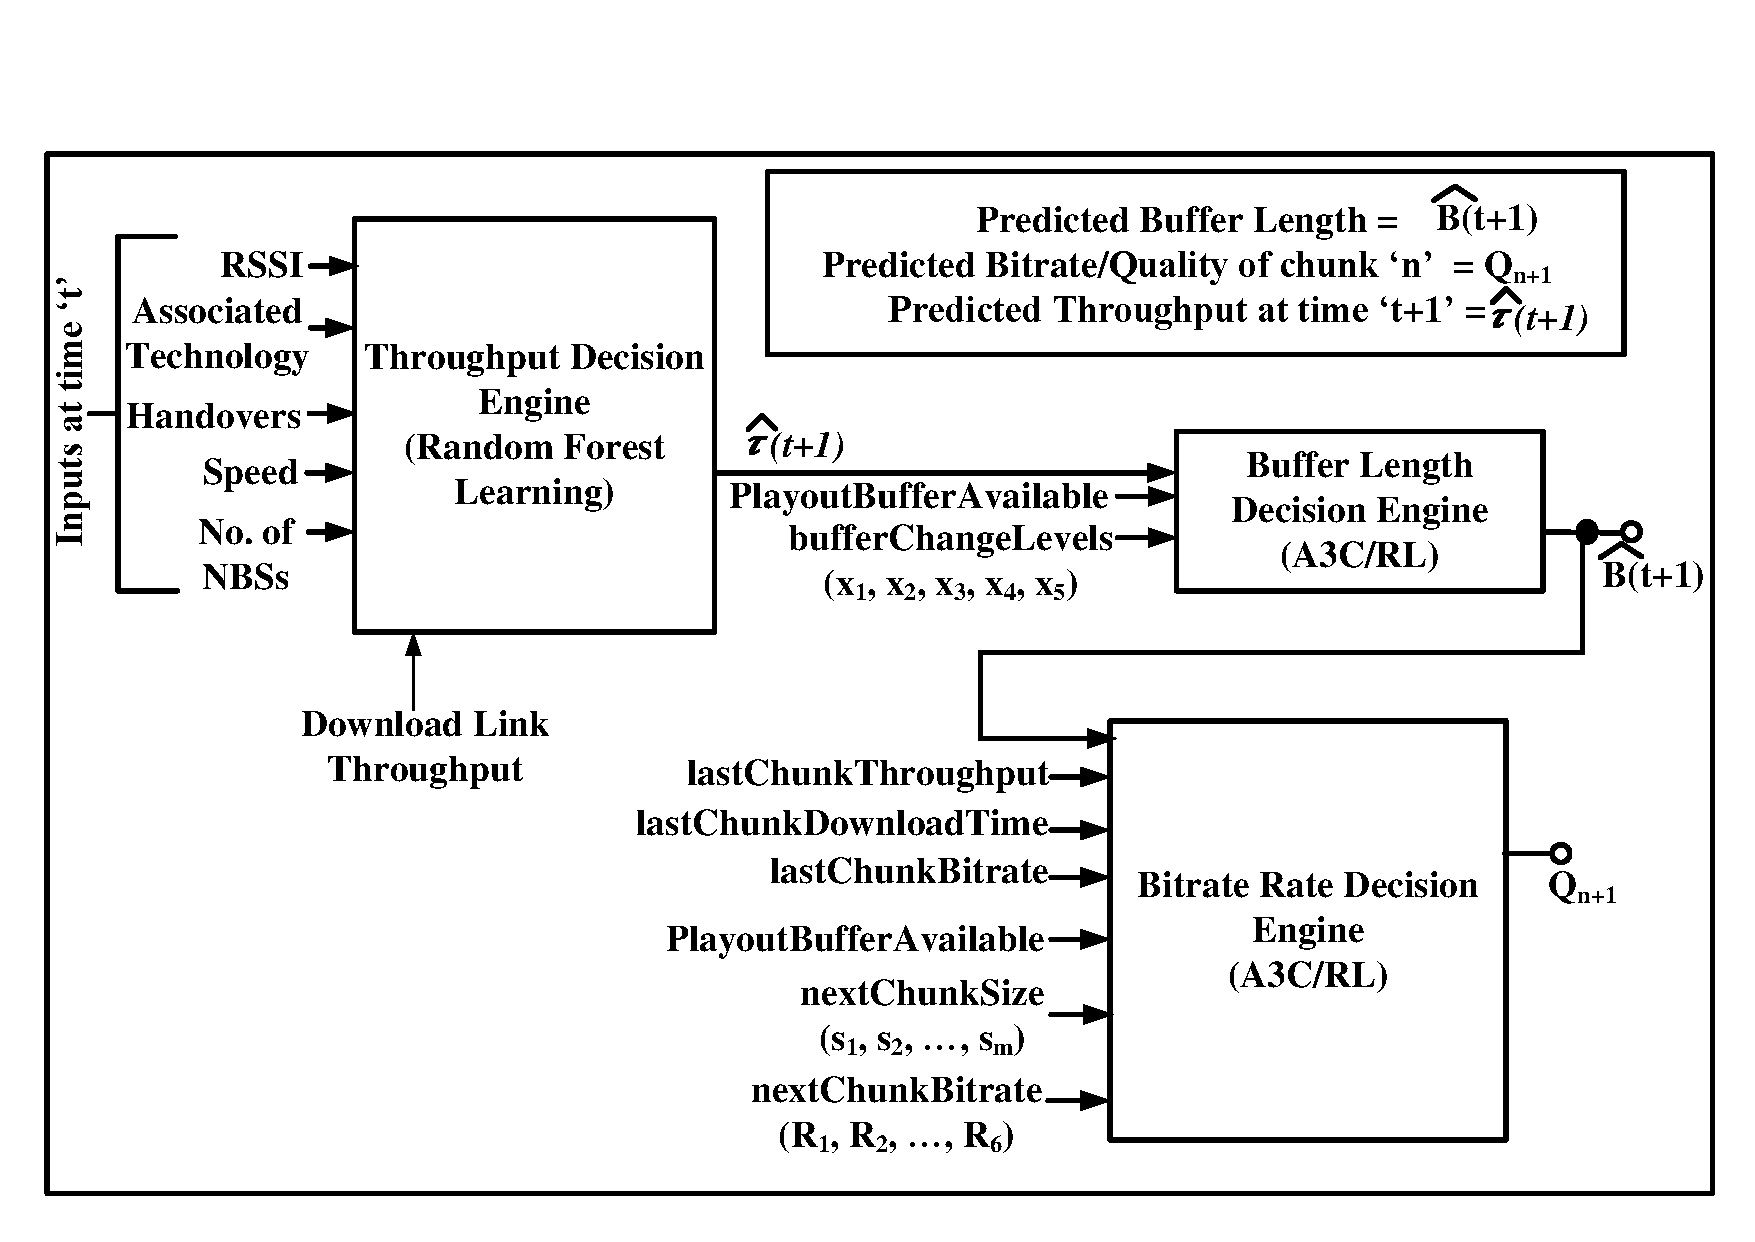
\includegraphics[width = 0.7\textwidth,trim = {1cm 1cm 1cm 1cm}]{figures/EnDASH_system.pdf}
	\caption{Composite Representation of the EnDASH model; a cascaded model where the predicted throughput acts as an input network state to the Actor Critic \ac{RL} based decision engine}
	\label{fig:chap04:EnDASH system}
\end{figure}

\subsection{The Throughput Prediction Engine}\label{sec:chap04:thpre}
EnDASH employs a \ac{RFL} algorithm for cellular network throughput prediction ~\cite{Raca2019}. At the beginning of time slot \mq{t}, it uses the historical information of different radio related parameters in the previous \mq{x} seconds to predict the average throughput~\footnote{Since video rate adaptation algorithms mostly use average throughput, hence for EnDASH, we have predicted the average throughput only \cite{Raca2019}.} that may be experienced by the user during the time slot (of length `T'). We represent this as $\prefu{x}{T}$.
The input features of the throughput prediction engine are: (i) \ti{RSSI}, (b) \ti{technologies used} - LTE (4G), HSPA+ (3.75G), UMTS (3G), EDGE (2G), (c) \ti{number of vertical and horizontal \ti{handovers}}, (d) \ti{speed},  (e) \ti{number and technology of neighbouring \acp{BS}}, (f) \ti{download link throughput} - the download rate is measured at the \ac{UE} in bytes per second. Readings on these features  are obtained from the NetMonitor Lite app with a granularity of one second.

\indent  Each feature can be represented as a distribution,
However, instead of feeding the entire time-series data for each metric, we adopt the summarization technique of \cite{Raca2019}. So, we feed only a few key values that best summarize the data and its corresponding distribution.
For each of the features we obtain the $\mathrm{25^{th}}$, $\mathrm{75^{th}}$, and $\mathrm{90^{th}}$ percentile points, median and mean from its historical data and feed it to the \ac{RFL} algorithm. We train and test this module using 39662 seconds of collected data on received throughput across five Indian cities.
 
\subsection{The Buffer Length Decision Engine}\label{sec:chap04:buff_length_dec_engine}
\indent The Buffer Length Decision engine also runs at the beginning of each time slot and the playback buffer length is predicted from the predicted network throughput.  However, the relationship between the predicted throughput and the buffer length is not straightforward and is not analytically tractable. So, we employ an A3C \ac{RL} based deep neural network to determine the optimal buffer length.
 
\indent The components of the \ac{RL} algorithm corresponding to the buffer decision engine are as follows:\\
% \begin{itemize}
\noindent \textbf{(i) Environment}  \ti{E} - video player.\\
\noindent \textbf{(ii) Input state at timeslot \mq{t}} $S_t$ =  ($\hat{\tau}_{{t}}$, $B_{av_t}$, ${\mathcal{X}}$), where
  $\hat{\tau}_{{t}}$ is the  average predicted cellular network throughput,
 $B_{av_t}$ is the current playback buffer capacity available in seconds,
$\mathcal{X}$ is the set of possible changes in buffer length. If the current buffer length is $B_{t-1}$, the next buffer length can be predicted to be $\hat{B_t}= B_t+x$ where $x\in\mathcal{X}:=\{-2,-1,0,+1,+2\}$. $x=1$ implies an increase in buffer length by a single chunk.\\
%, each chunk is of eight seconds.\\
\noindent \textbf{(iii) Action} $A_t$ - Decisions on the increase or decrease of buffer length at timeslot $t$. \\
\noindent \textbf{(iv) Reward} - The reward function is defined as a linear weighted function of energy savings with respect to a baseline ABR algorithm and the QoE score:
    \begin{equation}
    \Xi_{\mathrm{bufflen}} = w_1 \cdot (\left|E_{\mathrm{EnDASH}_t}-E_{\mathrm{old}_t}\right|)+w_2 \cdot QoE
    \end{equation}

\indent The first term in the reward function gives the energy savings with respect to a baseline ABR algorithm. In this work, we have chosen BOLA \cite{Spiteri2016} as the baseline since its energy consumption is the lowest among existing algorithms (excluding EnDASH, \S{\ref{sec:chap04:evaluation}}).  $E_{\mathrm{old}_t}$ and $E_{\mathrm{EnDASH}_t}$ represent the energy consumption of BOLA and of EnDASH at time \mq{t}, respectively. The energy consumed while using one particular algorithm is obtained as follows:  the RRC states are first identified from the download packet capture of a video trace. Next, the dwell time in each RRC state is multiplied by the corresponding power consumption (obtained from the RRC state machine) to get the energy quantities. We calculate the energy savings in this manner because the ground truth on energy consumption cannot be obtained.

\indent Second term in the reward function is the \textbf{\ac{QoE}} metric  \cite{yin2015control}:
\begin{equation}\label{eq:chap04:QoE}
   \text{QoE} = \sum_{i=1}^N q(R_i) - \mu\sum_{i=1}^N \delta_i - \sum_{i=1}^{N-1}\left|q(R_{i+1})-q(R_i)\right|
\end{equation}
The $\text{QoE}$ metric is defined for a video with N chunks. $R_i$ is the bitrate of $\text{chunk}_i$ and $q(R_i)$ maps the bitrate to a quantity which represents the quality perceived by the user. We have taken $q(R_i) = R_i$ \cite{mao2017neural}. $\delta_i$ is the rebuffering time involved in downloading $\text{chunk}_i$ at bitrate $R_i$. $\mu$ represents the degree of penalty associated with $\delta_i$.  We have taken $\mu=4.3$ \cite{mao2017neural}. The last term represents the playback smoothness. The QoE decreases when there is abrupt variability in throughput between successive chunks. Thus, QoE increases with bitrate, and reduces with rebuffering time and throughput variability.
\subsection{The Bitrate Decision Engine}
 \label{sec:chap04:bitrate_dec_engine} 
The predicted playback buffer length is next used for selecting optimal chunk bitrates using a deep \ac{RL} based algorithm. The components of the \ac{RL} algorithm are:\\

\noindent\textbf{(i) Environment}  \ti{E} - video player.\\
\noindent\textbf{(ii) Input state before downloading the chunk \mq{n}}, \\$S_{n}$ = ($\hat{\mathcal{B}_t}, \tau_c(n-1)$, $d_{n-1}$, $l_{n-1}$, $B_{n}$, $\zeta_{n}$, $r_{n}$), where $\hat{\mathcal{B}_t}$- predicted playback buffer length for current slot \mq{t}, $\tau_c(n-1)$= throughput of last chunk, $d_{n-1}$ = time taken to download last chunk, $l_{n-1}$ = bitrate of last chunk, $B_{n}$ = available playback buffer length, $\zeta_{n}\in\bracket{s_1,s_2,\cdots s_m}$ = Possible size of next video chunk  ($m$ available sizes), $r_{n+1}\in \bracket{R_1, R_2,\cdots, R_6}$ = Possible bitrate levels for next video chunk.\\
\noindent\textbf{(iii) Action} $A_n$ - Optimal bitrate decision for the next chunk.\\ 
\noindent\textbf{(iv) Reward}- QoE score obtained from \eqn\ref{eq:chap04:QoE}.\\
\indent The buffer length and bitrate decision engines run at two different time scales. So, time slot indices for the variables related to the buffer length decision engine and the bitrate decision engine are denoted by  \mq{t} and \mq{n}, respectively.

\section{Emulation environment for \ac{RL} training}
In the training phase, the \ac{RL} agent of the buffer and the bitrate decision engine of EnDASH should ideally be trained using real video downloads at actual video streaming clients. 
However, this demands that entire chunks be downloaded for each training data point. Further, downloads over cellular networks can be quite slow. Hence, to save training time, we train EnDASH and its competing  ABR algorithms using an emulation environment that closely mimics a real video client application. The emulator maintains its own representation of a real client's playback buffer. At the beginning of a time slot, the emulator first predicts the average throughput and then the playback-buffer length for the slot. Within the slot, once a chunk is to be downloaded, the emulator first assigns a download time to the chunk based  on its bitrate and the internal network throughput, derived from previous chunks. It then depletes the playback-buffer by the chunk's download time to emulate the playback-buffer drainage during an ongoing chunk download. It adds the playback duration of the  chunk being currently downloaded to the playback-buffer. The emulator sleeps temporarily once the playback buffer is full. Rebuffering occurs if the playback-buffer is completely drained before the next chunk download. The emulator keeps track of the rebuffering event and rebuffering time. After each slot (chunk download), the emulator prepares the state $S_t$ ($S_n$) for the \ac{RL} module of the buffer decision (bitrate decision) engines.
\subsection{The \ac{RL} Training algorithm}
Both the buffer length and bitrate decision engines of EnDASH are trained using  state-of-the-art actor-critic method, which involves training two neural networks \cite{mao2017neural}: an actor network and a critic network. A3C is a policy gradient \ac{RL} algorithm which estimates the gradient of the total reward from the trajectories of the execution followed by a policy. The action is chosen based on the policy by the actor network while the critic network estimates the advantage of selecting the action by returning a value function. Both networks update their weights in each time step.
 
\indent Each parameter of the state \ti{S} of both buffer length and bitrate decision engines are passed on to their respective actor and critic network to enable learning of optimal buffer lengths and bitrates by the corresponding \ac{RL} modules~\cite{mao2017neural}.
As in \cite{mao2017neural}, we initiate multiple learning agents to accelerate the training. By default, there are 16 agents. Each agent is designed to experience a different set of input parameters, e.g., network traces. However, the learning agents continuously report  their individual tuples of (state, action, reward)  to a central model, which aggregates them to generate a single model.
\subsection{Implementation of the \ac{RL} modules}
The \textit{bitrate selection engine} of EnDASH is adopted from the state-of-the-art Pensieve algorithm \cite{mao2017neural}, which also uses A3C to learn optimal bitrates. We have used a pretrained model provided by Pensieve, albeit with different input states.  The \textit{buffer length decision engine} has been implemented in Tensorflow \cite{Abadi2016}. The engine passes five previous values of the buffer length to a 1D convolution layer (CNN) with 128 filters, each of size 4 with stride 1. The remaining inputs, i.e., predicted link throughput and current available buffer length are passed onto another 1D-CNN having the same shape. Results obtained from these layers are subsequently combined in a hidden layer having 128 neurons and uses the softmax function. The same inputs are also used by the critic network, which has the same neural network, but whose final output is a linear neuron. During the training of the algorithm, we set the discount factor to 0.9, i.e., current actions are allowed to be influenced by 100 future steps. The learning rates for the actor and the critic networks are 0.0001 and 0.001, respectively. The entropy factor $\beta$ has been set to gradually decrease from 1 to 0.1 over iterations.
